\documentclass{article}
\usepackage[utf8]{inputenc}
\usepackage{graphicx}
\usepackage{float}
\usepackage{multirow}
\usepackage{booktabs}
\usepackage{wrapfig}
\usepackage{amsmath}
\graphicspath{ {images/} }
\usepackage{hyperref}
\hypersetup{
    colorlinks=true,
    linkcolor=blue,
    filecolor=magenta,      
    urlcolor=cyan,
}
 
\urlstyle{same}



\title{Box2D Project Description}
\author{ Group-33 }
\date{August 2015}

\begin{document}

\maketitle

\begin{table}[h!]
\begin{center}

 \begin{tabular}{*{3}{c}}
\toprule
Group Name & Name & Roll No.\\
\midrule
\multirow{3}{*}{Anonymous} & Deep & 140050002 \\
  & Kapil & 140050006 \\
  & Mohit & 140050015 \\
\bottomrule
\end{tabular} 
 
\end{center}
\end{table}




\newpage

\section{Motivation}
This project is prepared under cs251 ( Systems Lab ) course.

\section{Introduction}
\begin{itemize}
  \item This project is to design Rube-Goldberg machine.
  \item Subsequent sections will give the description for our design of the machine.
\end{itemize}

\section{Project Design}
Our project is basically a Box2D simulation of mechanical adder which is implemented with a Rube-Goldberg machine type setup. It counts the number of small balls present in container marked 8 (see figure below) . We can see number of balls present in a binary representation in part-11 of figure (see description below) .
\begin{figure}[h]
  \begin{center}
    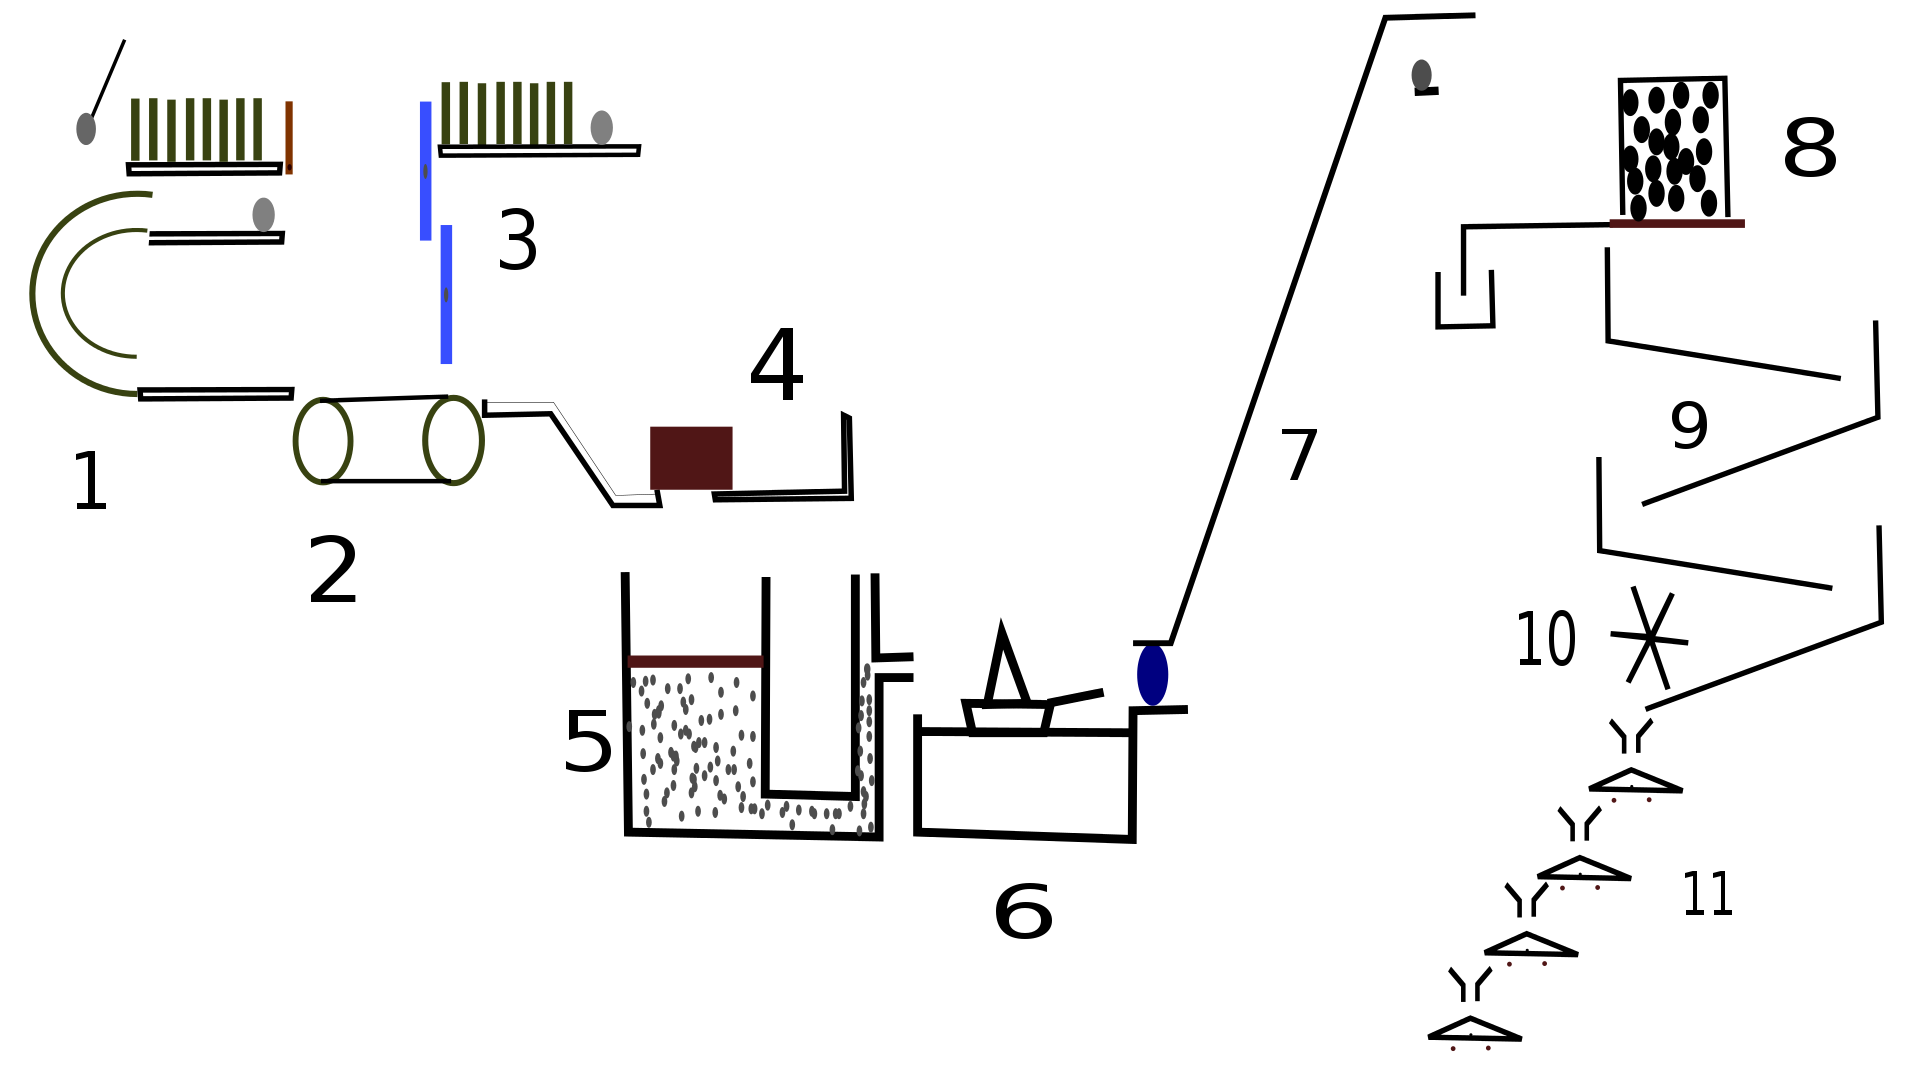
\includegraphics[width=1\textwidth]{projectfinalfinal}
  \end{center}
  \caption{Mechanical Adder}
\end{figure}

(see a real life mechanical adder in action \href{https://www.youtube.com/watch?v=GcDshWmhF4A}{here}\cite{youtube})

\newpage

\section{components}

\subsection{component-1}

\begin{wrapfigure}{r}{0.5\textwidth}
    \centering
    \vspace{-20pt}
    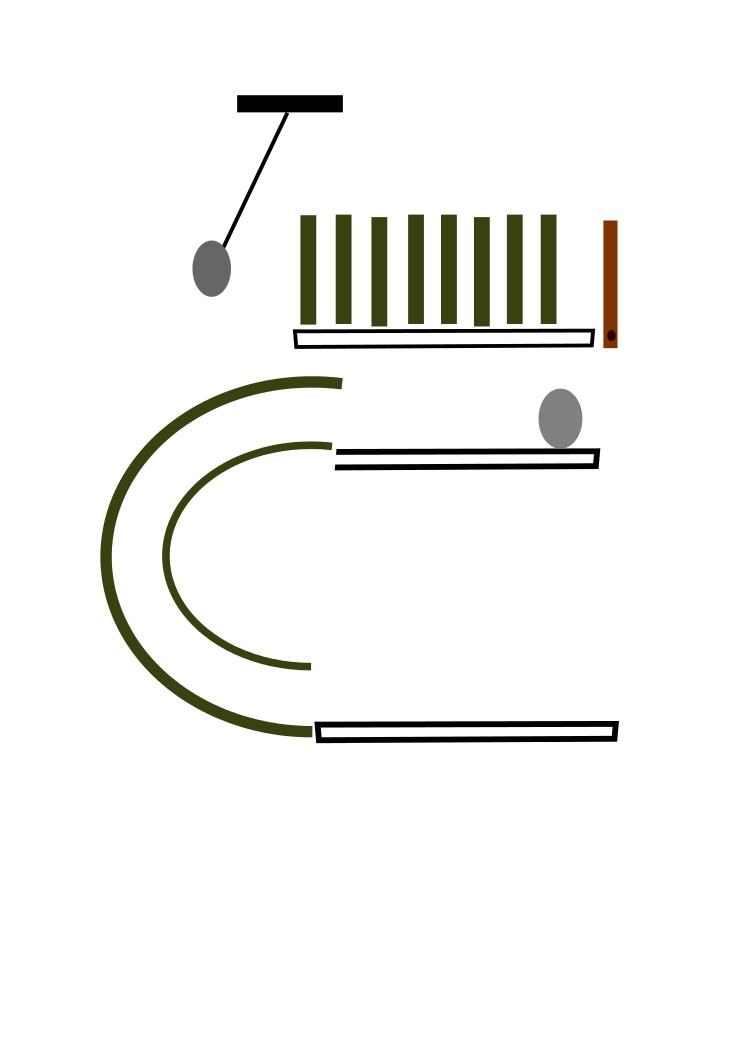
\includegraphics[width=0.18\textwidth]{newp1}
\end{wrapfigure}
Simulation of machine starts here. Initially swinging pendulum hits dominoes
which then rotate pivoted plank. The plank then hits the ball. 
Ball then travels through the tube .

\subsection{component-2}
This is a motor which gives ball coming from part-1 more speed , so as to improve the accuracy of simulation. (see figure one for whole image).\\
%\begin{wrapfigure}{l!}{0.3\textwidth}
%    \centering
%    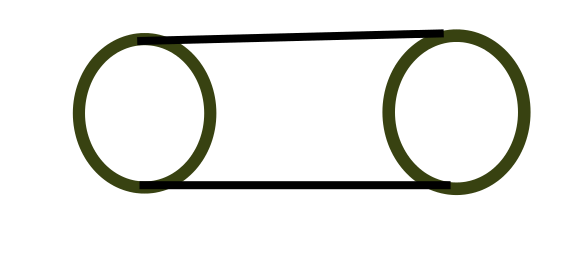
\includegraphics[width=0.18\textwidth]{p2}
%\end{wrapfigure}
\\


\subsection{component-3}

\begin{wrapfigure}{r}{0.5\textwidth}
    \centering
    \vspace{-20pt}
    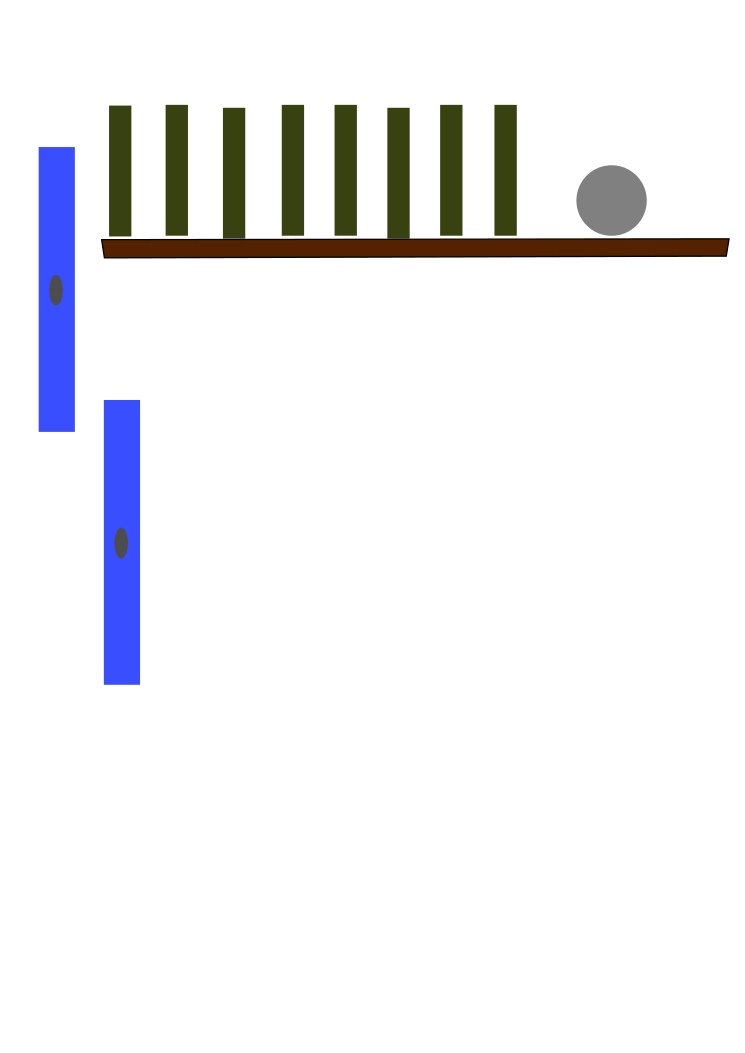
\includegraphics[width=0.18\textwidth]{p3}
\end{wrapfigure}
Moving ball then hits the rotating plates which disturbs the system of vertical blocks (Moving plates describe the concept of torque in classical mechanics\cite{eq2}) .They then drop the ball on the platform.\\
\\
\\

\subsection{component-4}

\begin{wrapfigure}{l}{0.5\textwidth}
    \centering
    \vspace{-20pt}
    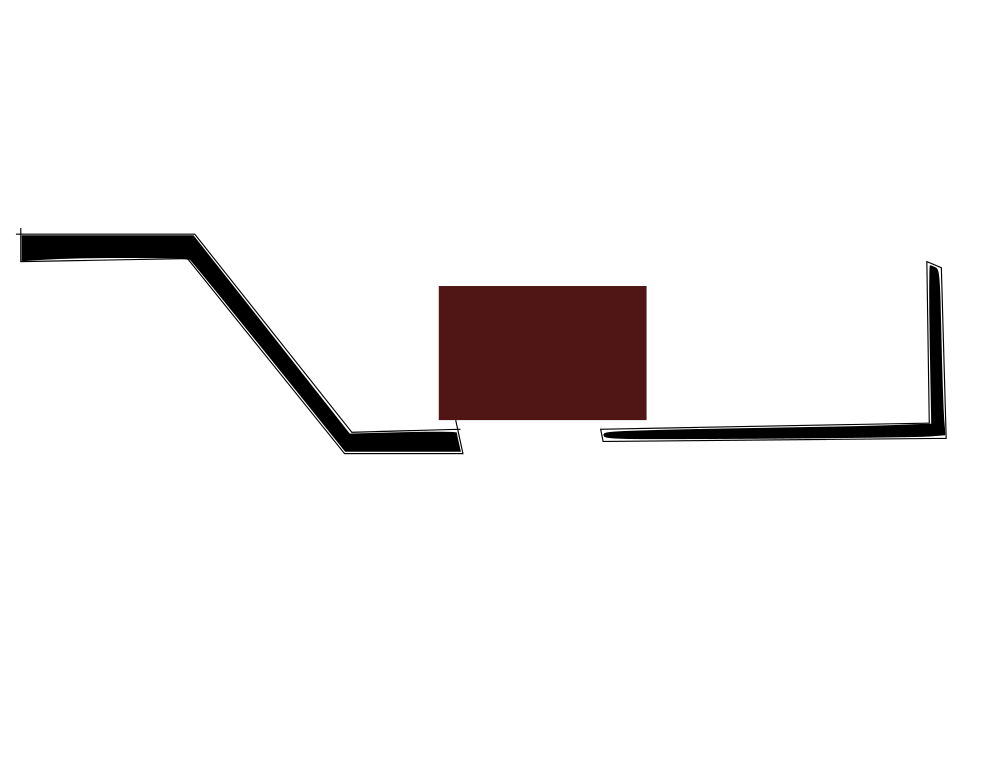
\includegraphics[width=0.18\textwidth]{p4}
\end{wrapfigure}
Moving ball from from component-2 hits the box to open the hole. 
\\
\\
\\

\newpage


\subsection{component-5}
This is a spray system which pushes the boat floating on liquid(see main figure).\\ 
\begin{wrapfigure}{r}{0.5\textwidth}
    \centering
    \vspace{-20pt}
    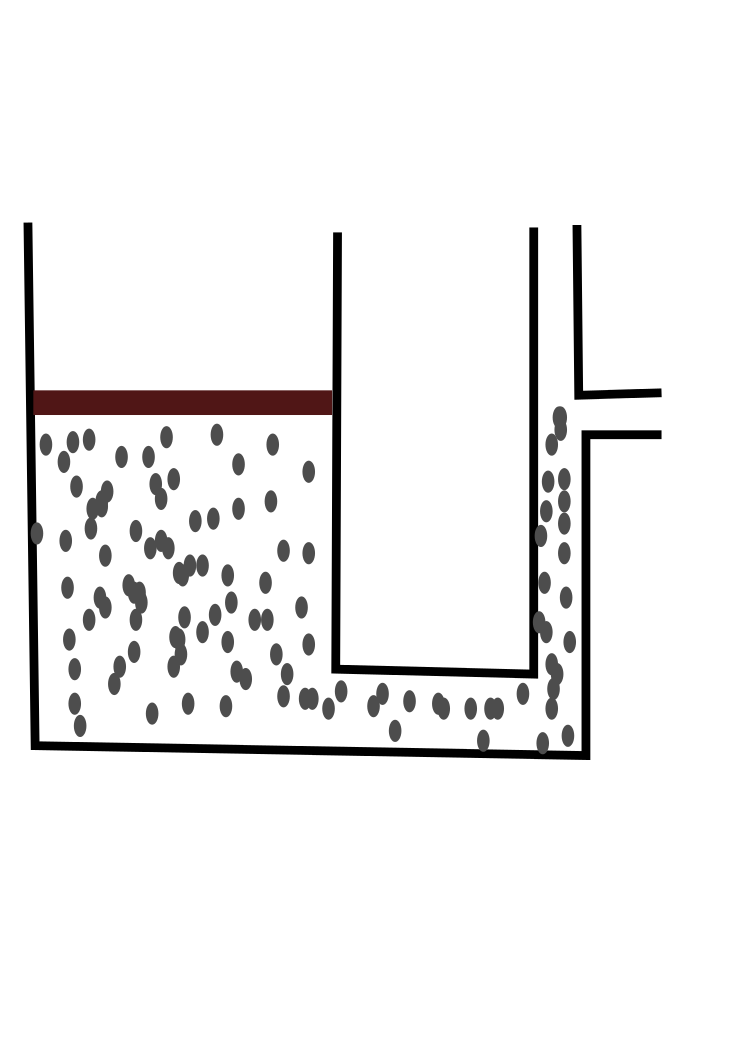
\includegraphics[width=0.18\textwidth]{p5}
    \vspace{-20pt}
\end{wrapfigure}
It consists of many small particles , resembling fluid , inside a container.
It runs on the principle of hydraulic lift (i.e. pascal's law)\cite{eq1}. When moving ball drops on the platform on the left , tiny particles are sprayed from right which then pushes the boat.
\\
\\
\\

\subsection{component-6}
\begin{wrapfigure}{l}{0.5\textwidth}
    \centering
    \vspace{-20pt}
    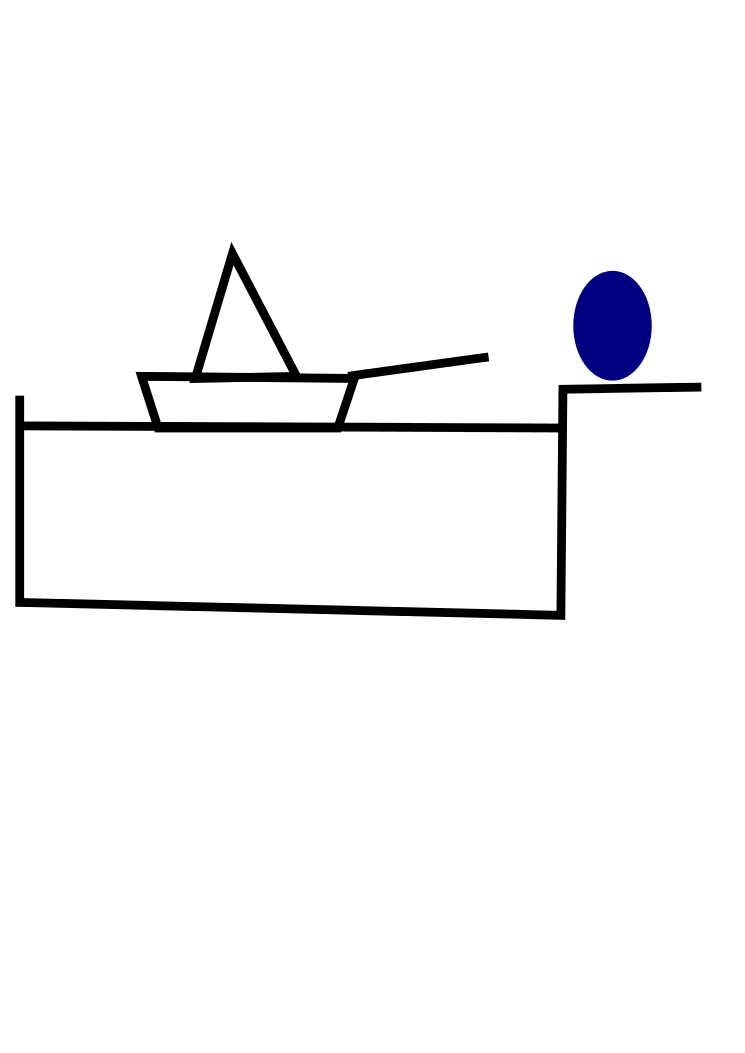
\includegraphics[width=0.18\textwidth]{p6}
    \vspace{-20pt}
\end{wrapfigure}
This part consists of a boat floating on liquid ( law of buoyancy is in action here ). When particles spayed by previous component hits this boat,
it pushes the balloon in its right side .
\\
\\
\\

\subsection{component-7}
\begin{wrapfigure}{r}{0.5\textwidth}
    \centering
    \vspace{-20pt}
    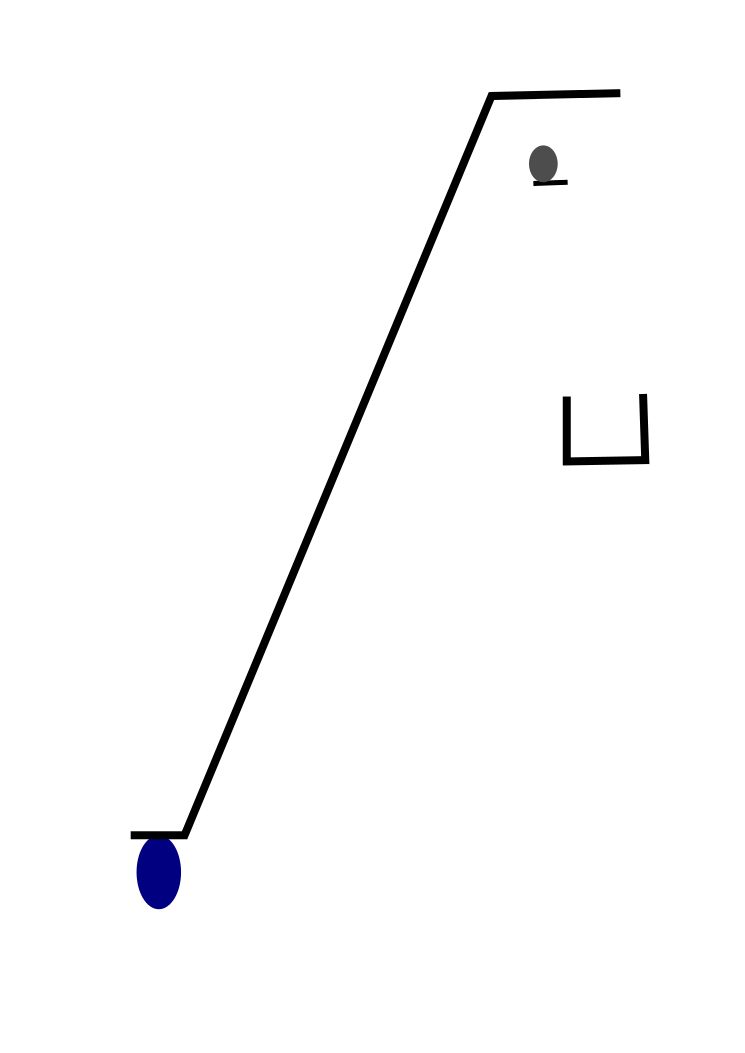
\includegraphics[width=0.18\textwidth]{p7}
    \vspace{-20pt}
\end{wrapfigure}
Moving balloon rises up, along the wedge , and pushes the ball to drop it.
\\
\\
\\
\\

\subsection{component-8}
\begin{wrapfigure}{l}{0.5\textwidth}
    \centering
    \vspace{-20pt}
    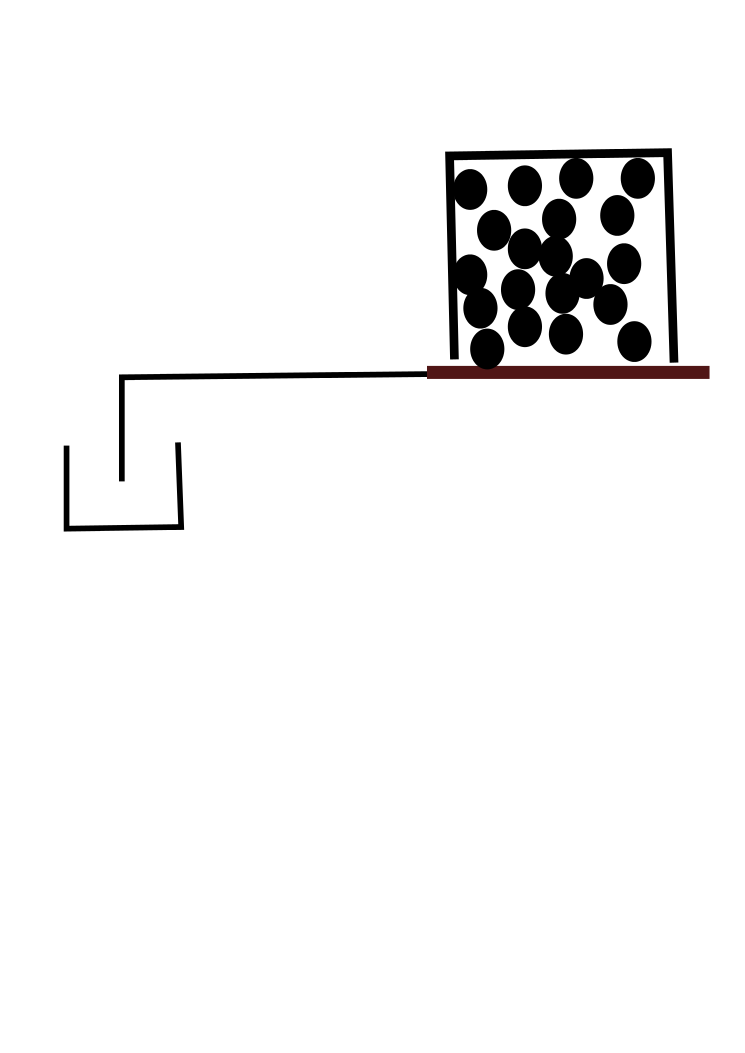
\includegraphics[width=0.18\textwidth]{p8}
    \vspace{-20pt}
\end{wrapfigure}
This part consists of a box containing some balls. We want to count the number of balls using the mechanical adder. Box is closed by a sliding lid .
when ball falls on the empty bucket (from previous setup ) , because of pulley system it opens the lid of the bow , thus balls starts falling onto the next component.
\\

\newpage

\subsection{component-9}
\begin{wrapfigure}{r}{0.5\textwidth}
    \centering
    \vspace{-20pt}
    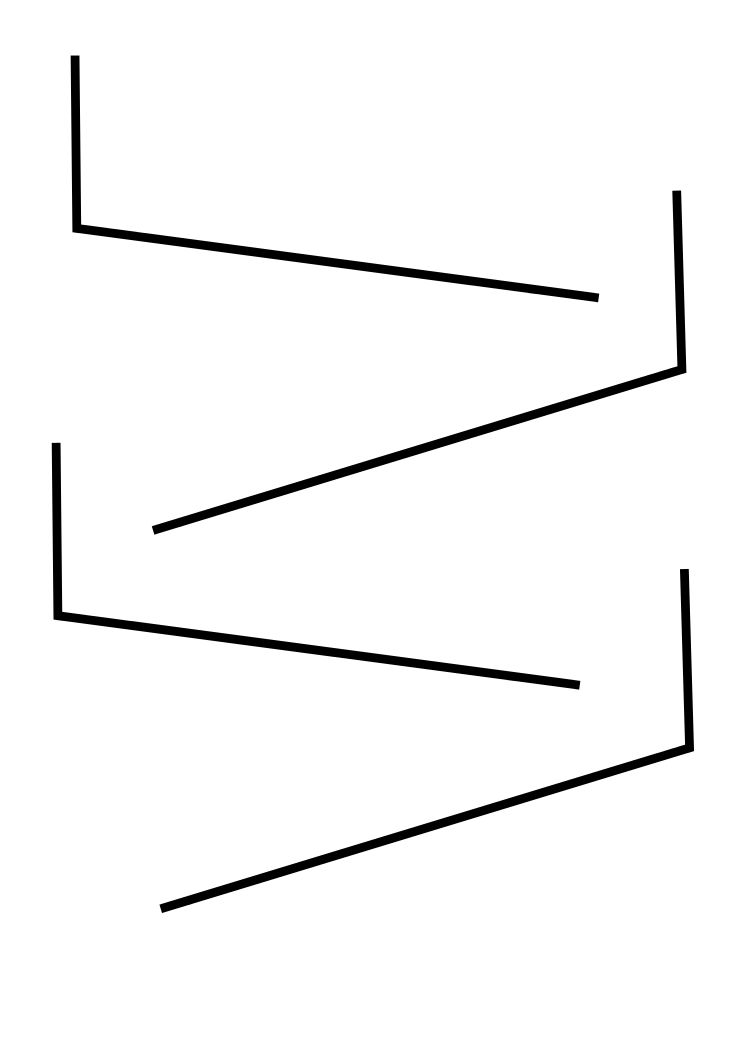
\includegraphics[width=0.18\textwidth]{p9}
    \vspace{-20pt}
\end{wrapfigure}
The zig-zag path make sure that balls fall into the adder in a single line
and not all once.
\\
\\
\\

\subsection{component-10}
\begin{wrapfigure}{l}{0.5\textwidth}
    \centering
    \vspace{-20pt}
    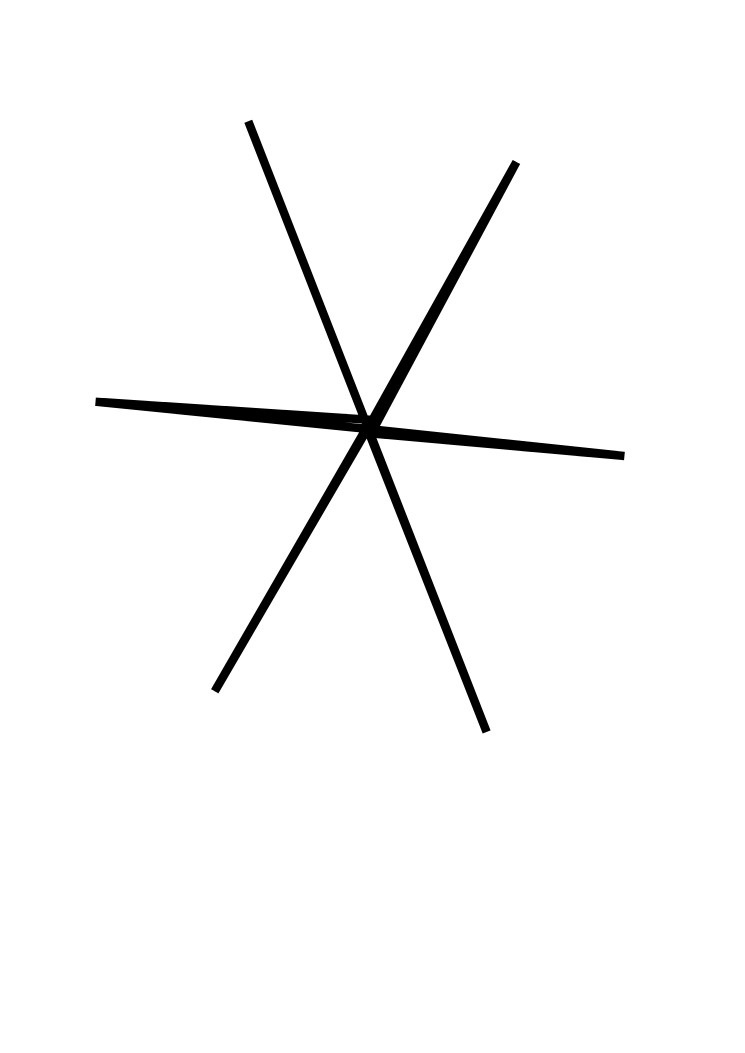
\includegraphics[width=0.18\textwidth]{p10}
    \vspace{-20pt}
\end{wrapfigure}
This component is a rotating wheel which act as a 'separator' ,i.e. it make sure that balls fall inside the adder with a certain time gap so that we get an accurate estimate of number of balls inside the above box. 
\\
\\
\\

\subsection{component-11}
\begin{wrapfigure}{r}{0.5\textwidth}
    \centering
    \vspace{-20pt}
    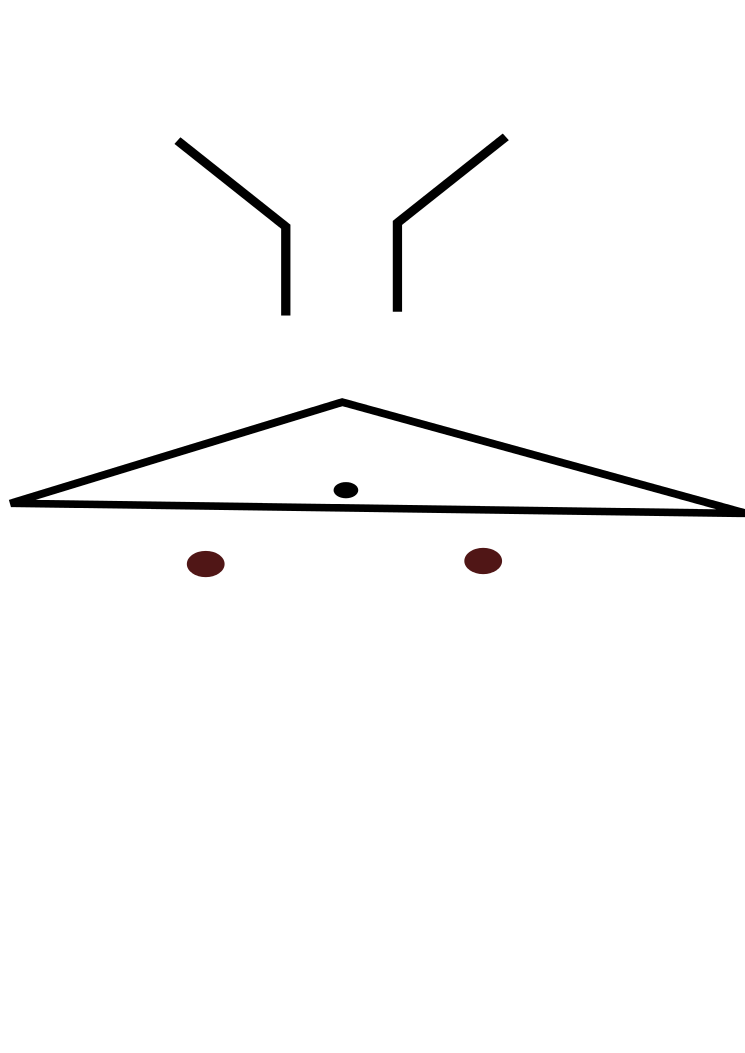
\includegraphics[width=0.18\textwidth]{p11}
    \vspace{-20pt}
\end{wrapfigure}
This part consists of a series of pivoted triangles which will work as the 'adder'. There are only two possible configuration of a triangle (i.e left and right rotated). From left to right , configuration of each triangle signifies the bit of the binary representation of the number which the whole system represents (right means 0 and left means 1).Thus by observing the final configuration of triangles we can calculate the number of balls which must have passed through it , thereby counting the number of balls in the box numbered 8 in the main diagram.
\\
\\
\\

\newpage

\section{Conclusion}
We hope you like our project in action when it is completed in future.
\\
\\
\\

\bibliographystyle{plain}
\bibliography{references}



\end{document}
